\caulc
%%%=============EX_1=============%%%
\begin{ex}%[2D4N1-3]%[TDMZZ06]%[Mui Doan]
	Nguyên hàm của hàm số $y = \dfrac{1}{\sin^2 x}$ là
	\choice
	{\True $-\cot x + C$}
	{$\cot x + C$}
	{$-\cos x + C$}
	{$-\dfrac{1}{\sin x} + C$}
	\loigiai{
		Ta có $\displaystyle\int \dfrac{1}{\sin^2 x}\mathrm{\,d}x=-\cot x + C$.
	}
\end{ex}
%%%=============================%%%

%%%=============EX_2=============%%%
\begin{ex}%[2D4H3-2]%[TDMZZ06]%[Huỳnh Trí Thiện]
	Cho hình phẳng $(H)$ giới hạn bởi các đường $y=6x-x^2$, $y=0$. Hãy tính thể tích khối tròn xoay thu được khi cho $(H)$ quay quanh trục hoành $Ox$.
	\choice
	{\True $\dfrac{1\,296\pi}{5}$}
	{$36$}
	{$\dfrac{1\,296}{5}$}
	{$36\pi$}
	\loigiai{
		Phương trình hoành độ giao điểm của $y=6x-x^2$ và $y=0$ là
		\[ 6x - x^2 = 0 \Leftrightarrow \hoac{&x = 0 \\ &x = 6.} \]
		Thể tích khối tròn xoay thu được khi quay hình $(H)$ quanh trục $Ox$ là
		\[ V = \pi \int\limits_{0}^{6} \left( 6x - x^2 \right)^2 \mathrm{\,d}x = \pi \int\limits_{0}^{6} \left( 36x^2 - 12x^3 + x^4 \right) \mathrm{\,d}x= \dfrac{1\,296\pi}{5}. \]
		Vậy thể tích cần tìm là $V = \dfrac{1\,296\pi}{5}$.
	}
\end{ex}
%%%=============================%%%

%%%=============EX_3=============%%%
\begin{ex}%[2D3H2-2]%[TDMZZ06]%[Unknown]
	Cho hai mẫu số liệu ghép nhóm $M_1$, $M_2$ với bảng tần số ghép nhóm:
	\begin{center}
		\begin{tabular}{cc}
			$M_1$ &
			\begin{tabular}{|c|c|c|c|c|c|c|}
				\hline
				Nhóm & $[2;3)$ & $[3;4)$ & $[4;5)$ & $[5;6)$ & $[6;7)$ & $[7;8)$ \\
				\hline
				Tần số & $5$ & $4$ & $6$ & $4$ & $2$ & $4$ \\
				\hline
			\end{tabular}
		\end{tabular}
	\end{center}
	\begin{center}
		\begin{tabular}{cc}
			$M_2$ &
			\begin{tabular}{|c|c|c|c|c|c|c|}
				\hline
				Nhóm & $[2;3)$ & $[3;4)$ & $[4;5)$ & $[5;6)$ & $[6;7)$ & $[7;8)$ \\
				\hline
				Tần số & $10$ & $8$ & $12$ & $8$ & $4$ & $8$ \\
				\hline
			\end{tabular}
		\end{tabular}
	\end{center}
	Gọi $s_1$, $s_2$ lần lượt là độ lệch chuẩn của hai mẫu số liệu $M_1$, $M_2$. Đáp án so sánh \textbf{đúng} là:
	\choice
	{$s_1 > s_2$}
	{\True $s_1 = s_2$}
	{$s_1 = 2s_2$}
	{$s_1 < s_2$}
	\loigiai{
		Ta có bảng giá trị đại diện của các nhóm số liệu:
		\begin{center}
			\begin{tabular}{|c|c|c|c|c|c|c|}
				\hline
				Nhóm & $[2;3)$ & $[3;4)$ & $[4;5)$ & $[5;6)$ & $[6;7)$ & $[7;8)$ \\
				\hline
				Giá trị đại diện ($x_i$) & $2{,}5$ & $3{,}5$ & $4{,}5$ & $5{,}5$ & $6{,}5$ & $7{,}5$ \\
				\hline
				Tần số $M_1$ ($m_i$) & $5$ & $4$ & $6$ & $4$ & $2$ & $4$ \\
				\hline
				Tần số $M_2$ ($m'_i$) & $10$ & $8$ & $12$ & $8$ & $4$ & $8$ \\
				\hline
			\end{tabular}
		\end{center}
		\textbf{Xét mẫu số liệu $M_1$:}
		
		Cỡ mẫu $n_1 = 5 + 4 + 6 + 4 + 2 + 4 = 25$.
		
		Số trung bình của mẫu $M_1$ là:
		$$ \overline{x}_1 = \frac{5\cdot 2{,}5 + 4\cdot 3{,}5 + 6\cdot 4{,}5 + 4\cdot 5{,}5 + 2\cdot 6{,}5 + 4\cdot 7{,}5}{25} = 4{,}74. $$
		
		Phương sai của mẫu $M_1$ là:
		$$ s_1^2 = \frac{5(2{,}5 - 4{,}74)^2 + 4(3{,}5 - 4{,}74)^2 + \ldots + 4(7{,}5 - 4{,}74)^2}{25} = 2{,}8224. $$
		
		Suy ra độ lệch chuẩn $s_1 = \sqrt{2{,}8224} = 1{,}68$.
		
		\textbf{Xét mẫu số liệu $M_2$:}
		
		Nhận thấy tần số của mỗi nhóm trong mẫu $M_2$ đều gấp đôi tần số của nhóm tương ứng trong mẫu $M_1$ ($m'_i = 2m_i$). Do đó cỡ mẫu $n_2 = 2n_1 = 50$.
		
		Số trung bình của mẫu $M_2$ là:
		$$ \overline{x}_2 = \frac{\sum (2m_i)x_i}{2n_1} = \frac{2\sum m_i x_i}{2n_1} = \frac{\sum m_i x_i}{n_1} = \overline{x}_1 = 4{,}74. $$
		
		Phương sai của mẫu $M_2$ là:
		$$ s_2^2 = \frac{\sum (2m_i)(x_i - \overline{x}_2)^2}{2n_1} = \frac{2\sum m_i(x_i - \overline{x}_1)^2}{2n_1} = \frac{\sum m_i(x_i - \overline{x}_1)^2}{n_1} = s_1^2. $$
		
		Do phương sai bằng nhau nên độ lệch chuẩn cũng bằng nhau: $s_1 = s_2$.
	}
\end{ex}
%%%=============================%%%

%%%=============EX_4=============%%%
\begin{ex}%[2H5N1-3]%[TDMZZ06]%[Nguyễn Tấn Linh]
	Trong không gian $Oxyz$, phương trình tổng quát của mặt phẳng $(\alpha)$ có véc-tơ pháp tuyến $\overrightarrow{n}=(2;2;-1)$ và đi qua điểm $A(2;1;0)$ là
	\choice
	{$(\alpha)\colon 2x+2y-z+6=0$}
	{$(\alpha)\colon 2x+y-5=0$}
	{$(\alpha)\colon 2x+2y-z-3=0$}
	{\True $(\alpha)\colon 2x+2y-z-6=0$}
	\loigiai{
		Mặt phẳng $(\alpha)$ đi qua điểm $A(2;1;0)$ và có vectơ pháp tuyến $\overrightarrow{n}=(2;2;-1)$ có phương trình là
		\[2(x-2)+2(y-1)-1(z-0)=0 \Leftrightarrow 2x+2y-z-6=0.\]
	}
\end{ex}
%%%=============================%%%

%%%=============EX_5=============%%%
\begin{ex}%[1H8H1-2]%[TDMZZ06]%[Phạm Hải Dương]
	\immini[thm]{ Cho hình lập phương $ABCD. A'B'C'D'$. Hỏi cặp đường thẳng nào dưới đây \textbf{không} vuông góc với nhau?
		\choice
		{\True $AB$, $C'D'$}
		{$AC$, $B'D'$}
		{$AB'$, $CD'$}
		{$AC$, $BD'$}}{ 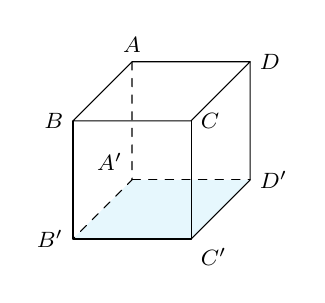
\begin{tikzpicture}[scale=1.5, line join=round, line cap=round,font=\footnotesize]
			% Các đỉnh đáy trên
			\coordinate (A) at (0.5,1.5);
			\coordinate (B) at (0,1);
			\coordinate (C) at (1,1);
			\coordinate (D) at (1.5,1.5);
			% Các đỉnh đáy dưới
			\coordinate (Ap) at (0.5,0.5);
			\coordinate (Bp) at (0,0);
			\coordinate (Cp) at (1,0);
			\coordinate (Dp) at (1.5,0.5);
			
			% Tô màu mặt đáy dưới
			\fill[cyan!10] (Bp) -- (Cp) -- (Dp) -- (Ap) -- cycle;
			
			% Vẽ các cạnh khuất
			\draw[dashed] (A) -- (Ap) -- (Bp);
			\draw[dashed] (Ap) -- (Dp);
			
			% Vẽ các cạnh còn lại
			\draw (A) -- (B) -- (C) -- (D) -- cycle;
			\draw (B) -- (Bp) -- (Cp) -- (C);
			\draw (D) -- (Dp) -- (Cp);
			
			% Tên các đỉnh
			\node[above] at (A) {$A$};
			\node[left] at (B) {$B$};
			\node[right] at (C) {$C$};
			\node[right] at (D) {$D$};
			\node[above left] at (Ap) {$A'$};
			\node[left] at (Bp) {$B'$};
			\node[below right] at (Cp) {$C'$};
			\node[right] at (Dp) {$D'$};
	\end{tikzpicture}}
	\loigiai{
		Xét từng phương án.
		\begin{itemize}
			\item $AB \parallel C'D'$ nên không thể vuông góc.
			\item $AC \parallel A'C'$ và $A'C' \perp B'D'$ (hai đường chéo hình vuông), suy ra $AC \perp B'D'$.
			\item $AB' \perp A'B$ (hai đường chéo hình vuông) và $A'B \parallel D'C$, suy ra $AB' \perp CD'$.
			\item $AC$ và $BD'$ vuông góc với nhau vì $AC\perp (BDD'B')$.
		\end{itemize}
		
	}
\end{ex}
%%%=============================%%%

%%%=============EX_6=============%%%
\begin{ex}%[2D1N4-1]%[TDMZZ06]%[Nguyễn Sơn Thành]
	Tổng số đường tiệm cận đứng và tiệm cận ngang của đồ thị hàm số $y = \dfrac{x^2 + 2x + 1}{x - 1}$ là
	\choice
	{\True $1$}
	{$2$}
	{$3$}
	{$0$}
	\loigiai{
		Xét hàm số $y = \dfrac{x^2 + 2x + 1}{x - 1}$.
		\begin{itemize}
			\item \textbf{Tiệm cận đứng:} Nghiệm của mẫu số là $x = 1$.\\ Ta có $\displaystyle \lim_{x \to 1^+} \dfrac{x^2 + 2x + 1}{x - 1} = +\infty$ và $\displaystyle \lim_{x \to 1^-} \dfrac{x^2 + 2x + 1}{x - 1} = -\infty$.\\ Suy ra đường thẳng $x = 1$ là tiệm cận đứng.
			\item \textbf{Tiệm cận ngang:} Ta có $\displaystyle \lim_{x \to \pm \infty} \dfrac{x^2 + 2x + 1}{x - 1} = \pm \infty$.\\ Suy ra đồ thị hàm số không có tiệm cận ngang.
		\end{itemize}
		Vậy tổng số đường tiệm cận đứng và tiệm cận ngang là $1$.
	}
\end{ex}
%%%=============================%%%

%%%=============EX_7=============%%%
\begin{ex}%[1D6H4-5]%[TDMZZ06]%[Bồ Văn Hậu]
	Tập nghiệm của bất phương trình $\ln (2x-4)<\ln (x+1)$ là
	\choice
	{$\{2;5\}$}
	{\True $(2;5)$}
	{$(5;+\infty)$}
	{$(-\infty;5)$}
	\loigiai{
		Điều kiện xác định $\heva{&2x-4>0\\&x+1>0}\Leftrightarrow \heva{&x>2\\&x>-1}\Leftrightarrow x>2$.\\
		Khi đó
		\allowdisplaybreaks
		\begin{eqnarray*}
			&&\ln (2x-4)<\ln (x+1)\\
			&\Leftrightarrow&2x-4<x+1\\
			&\Leftrightarrow&x<5.
		\end{eqnarray*}
		So với điều kiện $x>2$, ta được $2<x<5$.\\
		Vậy tập nghiệm của bất phương trình đã cho là $S=(2;5)$.
	}
\end{ex}
%%%=============================%%%

%%%=============EX_8=============%%%
\begin{ex}%[2H5N2-2]%[TDMZZ06]%[Lê Phúc]
	Trong không gian $Oxyz$, cho đường thẳng $\Delta \colon \dfrac{x-1}{3}=\dfrac{y-2}{2}=\dfrac{z+2}{1}$. Hỏi vectơ nào dưới đây là một vectơ chỉ phương của đường thẳng $\Delta$?
	\choice
	{$\overrightarrow{u}_1=(2;1;3)$}
	{$\overrightarrow{u}_2=(1;2;-2)$}
	{$\overrightarrow{u}_3=(2;1;2)$}
	{\True $\overrightarrow{u}_4=(3;2;1)$}
	\loigiai{
		Một vectơ chỉ phương của $\Delta$ là $\overrightarrow{u}_4=(3;2;1)$.
	}
\end{ex}
%%%=============================%%%

%%%=============EX_9=============%%%
\begin{ex}%[1D6H4-4]%[TDMZZ06]%[Trần Văn Thiện]
	Số nghiệm thực của phương trình $2^{x^2}=4^{4x-4}$ là
	\choice
	{$0$}
	{$1$}
	{\True $2$}
	{ $3$}
	\loigiai{
		Ta có $2^{x^2}=4^{4x-4} \Leftrightarrow 2^{x^2}=2^{8x-8}\Leftrightarrow x^2-8x+8=0\Leftrightarrow x=4\pm 2\sqrt{2}$.\\
		Phương trình có hai nghiệm phân biệt, vậy số nghiệm thực là $2$.
	}
\end{ex}
%%%=============================%%%

%%%=============EX_10=============%%%
\begin{ex}%[1D2H2-5]%[TDMZZ06]%[Đình Nguyên]
	Cho ba số $a$, $b$, $c$ theo thứ tự lập thành một cấp số cộng có tổng bằng $15$. Giá trị của $b^2 - (a + c)$ bằng
	\choice
	{$-5$}
	{\True $15$}
	{$5$}
	{$10$}
	\loigiai{
		Vì ba số $a$, $b$, $c$ theo thứ tự lập thành một cấp số cộng nên ta có $a + c = 2b$.\\
		Tổng của ba số bằng $15$ nên $a + b + c = 15 \Leftrightarrow (a + c) + b = 15 \Leftrightarrow 2b + b = 15 \Leftrightarrow 3b = 15 \Leftrightarrow b = 5$.\\
		Suy ra $a + c = 2b = 10$.\\
		Vậy $b^2 - (a + c) = 5^2 - 10 = 15$.
	}
\end{ex}
%%%=============================%%%

%%%=============EX_11=============%%%
\begin{ex}%[2H2H1-3]%[TDMZZ06]%[Huynh Quốc Đạt]
	Trong không gian cho hình lập phương $ABCD. A'B'C'D'$. Đáp án nhận xét \textbf{đúng} là
	\choice
	{$\left(\overrightarrow{AC},\overrightarrow{DB}\right)=60^\circ$}
	{$\left(\overrightarrow{AC},\overrightarrow{AA'}\right)=45^\circ$}
	{$\left(\overrightarrow{AC},\overrightarrow{AC'}\right)=45^\circ$}
	{\True $\left(\overrightarrow{AC},\overrightarrow{D'C}\right)=60^\circ$}
	\loigiai{
		\immini{
			\begin{itemize}
				\item $\left(\overrightarrow{AC},\overrightarrow{DB}\right)=90^\circ$ (do $AC\perp BD$).
				\item $\left(\overrightarrow{AC},\overrightarrow{AA'}\right)=90^\circ$ (do $AC\perp AA'$).
				\item $\left(\overrightarrow{AC},\overrightarrow{AC'}\right)=\widehat{CAC'}\neq 45^\circ$ (do $\triangle ACC'$ vuông tại $C$ nhưng không cân).
				\item $\left(\overrightarrow{AC},\overrightarrow{D'C}\right)= \widehat{ACD'} = 60^\circ$ (do các vectơ cùng hướng về điểm $C$ và $\triangle ACD'$ đều vì có ba cạnh là ba đường chéo của các mặt hình lập phương, $AC = AD' = CD' = a\sqrt{2}$).
		\end{itemize}}{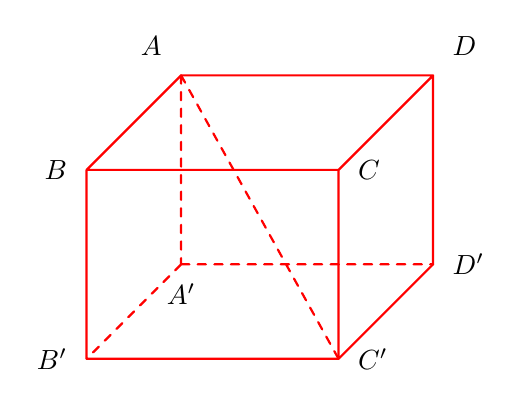
\begin{tikzpicture}[scale=0.8, line join=round, line cap=round]
				
				% Khai báo điểm (gọn)
				\foreach \name/\x/\y in {
					B/0/0, C/4/0, D/5.5/1.5, A/1.5/1.5,
					B'/0/-3, C'/4/-3, D'/5.5/-1.5, A'/1.5/-1.5
				}{
					\coordinate (\name) at (\x,\y);
				}
				% Vẽ cạnh
				\draw[thick, red] 
				(B)--(C)--(D)--(A)--cycle
				(B')--(C')--(D')
				(B)--(B') (C)--(C') (D)--(D');
				(D')--(C)--(A);
				
				% Nét đứt
				\draw[thick, red, dashed] (A)--(A') (A')--(D') (A')--(B') (A)--(C');
				
				\foreach \p/\g in {
					A/135, B/180, C/0, D/45,
					A'/-90, B'/180, C'/0, D'/0
				}{
					\node at (\p) [label=\g:$\p$] {};
				}
	\end{tikzpicture}}}
\end{ex}
%%%=============================%%%

%%%=============EX_12=============%%%
\begin{ex}%[2D1H5-7]%[TDMZZ06]%[Unknown]
	Đồ thị hàm số $y=\dfrac{x+3}{x-2}$ có tâm đối xứng cách gốc tọa độ một khoảng bằng
	\choice
	{$2$}
	{$1$}
	{\True $\sqrt{5}$}
	{$\sqrt{3}$}
	\loigiai{
		Ta có TCĐ $x=2$ và TCN $ y=1$.\\
		Do đó tâm đối xứng của đồ thị là giao điểm hai tiệm cận là
		$I(2;1)$.\\
		Khoảng cách từ $I$ đến gốc tọa độ $O(0;0)$ là
		$OI=\sqrt{(2-0)^2+(1-0)^2}=\sqrt{5}$.
	}
\end{ex}
%%%=============================%%%
\cauds
%%%=============EX_13=============%%%
\begin{ex}%[2D1H3-2]%[TDMZZ06]%[Dương Công Tạo]
	Cho hàm số $f(x) = x - 2\,026 \ln x$.
	\choiceTF
	{\True Tập xác định của hàm số là $(0;+\infty)$}
	{\True $f'(x)=1-\dfrac{2\,026}{x}$}
	{\True $f'(x) = 0 \Leftrightarrow x = 2\,026$}
	{\True Giá trị nguyên nhỏ nhất của hàm số bằng $-13\,399$}
	\loigiai{
		\begin{itemchoice}
			\itemch Tập xác định của hàm số $f(x) = x - 2\,026 \ln x$ là $(0;+\infty)$.
			\itemch Xét hàm số $f(x) = x - 2\,026 \ln x$ trên khoảng $(0;+\infty)$.\\
			Ta có $f'(x)=1-\dfrac{2\,026}{x}$.
			\itemch Ta có $f'(x)=1-\dfrac{2\,026}{x}=\dfrac{x-2\,026}{x}$; $f'(x)=0\Leftrightarrow x=2\,026$.
			\itemch Bảng biến thiên
			\begin{center}
				
\begin{tikzpicture}[>=stealth]
					\tkzTabInit[nocadre=false,lgt=1.5,espcl=3,deltacl=0.6]{$x$/.7 ,$f'(x)$/.7,$f(x)$/2}
					{$0$ , $2\,026$ , $+\infty$}
					\tkzTabLine{ d , - , 0 , + , }
					\tkzTabVar{D+/$+\infty$ , -/$2\,026 - 2\,026 \ln 2\,026$ , +/$+\infty$}
				\end{tikzpicture}
			\end{center}
			Dựa vào bảng biến thiên, ta có $\min\limits_{(0;+\infty)}f(x)=f(2\,026)=2\,026 - 2\,026 \ln 2\,026\approx -13\,399{,}60$.\\
			Vì hàm số liên tục trên khoảng $(0;+\infty)$ nên tập giá trị của hàm số là $[2\,026 - 2\,026 \ln 2\,026; +\infty)$.\\
			Vậy giá trị nguyên nhỏ nhất mà hàm số có thể đạt được là $-13\,399$.
		\end{itemchoice}
	}
\end{ex}
%%%=============================%%%

%%%=============EX_14=============%%%
\begin{ex}%[2D4V1-6]%[TDMZZ06]%[Hà Văn Hảo]
	Giả sử có một triều đại trong dã sử có nhà vua và $N_0$ quan thần trong một buổi thiết triều, nhà vua nêu ra một ý tưởng và hỏi ý kiến mọi người, cho phép tranh luận và thuyết phục nhau trong $2$ giờ, trong các quan thần bắt đầu chia làm hai phe, một phe ủng hộ và một phe phản đối, không tính đến nhà vua. Ngay lúc đầu đã có $20$ quan thần ủng hộ và bắt đầu ra sức thuyết phục phe còn lại. Biết tốc độ tăng số lượng quan thần ủng hộ $M'(t)$ tỉ lệ nghịch với số lượng quan thần hiện có của phe còn lại theo hằng số $k$, số lượng ủng hộ và phản đối lần lượt sau $t$ giờ là $M(t)$ và $N(t)$. Sau một giờ thuyết phục thì số lượng ủng hộ lên đến con số $30$, tiếp tục thuyết phục thêm $\dfrac{5}{7}$ giờ thì tăng thêm $10$ người nữa ủng hộ. Biết $\left\{[N(t)]^2\right\}' = 2N(t) \cdot N'(t)$.
	\choiceTF
	{\True $M(t) + N(t) = N_0$}
	{$N'(t) = \dfrac{k}{N(t)}$}
	{\True $k = 350$}
	{Số lượng người trong buổi thiết triều là $60$}
	\loigiai{
		\begin{itemchoice}
			\itemch Tổng số quan thần là không đổi trong suốt quá trình tranh luận, do đó số người ủng hộ $M(t)$ cộng với số người phản đối $N(t)$ luôn bằng tổng số quan thần ban đầu $N_0$.\\
			Vậy $M(t) + N(t) = N_0$.
			\itemch Theo giả thiết, tốc độ tăng số lượng người ủng hộ $M'(t)$ tỉ lệ nghịch với số lượng người phản đối $N(t)$ theo hằng số $k$, ta có $M'(t) = \dfrac{k}{N(t)}$.\\
			Vì $M(t) + N(t) = N_0$ (hằng số) nên đạo hàm hai vế theo $t$ ta được
			\[M'(t) + N'(t) = 0 \Rightarrow N'(t) = -M'(t) = -\dfrac{k}{N(t)}.\]
			\itemch Từ $N'(t) = -\dfrac{k}{N(t)}$, ta có $N(t) \cdot N'(t) = -k$.\\
			Lấy nguyên hàm hai vế theo $t$, ta được
			\[ \displaystyle\int N(t) \cdot N'(t) \mathrm{\,d}t = \displaystyle\int \left(-k\right) \mathrm{\,d}t \Rightarrow \dfrac{[N(t)]^2}{2} = -kt + C \Rightarrow [N(t)]^2 = -2kt + C_1.\]
			Tại thời điểm $t=0$, $M(0) = 20 \Rightarrow N(0) = N_0 - 20$. Do đó $C_1 = (N_0 - 20)^2$.\\
			Tại thời điểm $t=1$, $M(1) = 30 \Rightarrow N(1) = N_0 - 30$. Ta có
			\allowdisplaybreaks
			\begin{eqnarray*}
				&&(N_0 - 30)^2 = -2k(1) + (N_0 - 20)^2 \\
				&\Leftrightarrow& (N_0 - 30)^2 - (N_0 - 20)^2 = -2k \\
				&\Leftrightarrow& -20N_0 + 500 = -2k \\
				&\Leftrightarrow& k = 10N_0 - 250. \quad (1)
			\end{eqnarray*}
			Tại thời điểm $t = 1 + \dfrac{5}{7} = \dfrac{12}{7}$, $M\left(\dfrac{12}{7}\right) = 30 + 10 = 40 \Rightarrow N\left(\dfrac{12}{7}\right) = N_0 - 40$. Ta có
			\allowdisplaybreaks
			\begin{eqnarray*}
				& &(N_0 - 40)^2 = -2k\left(\dfrac{12}{7}\right) + (N_0 - 20)^2 \\
				&\Leftrightarrow& (N_0 - 40)^2 - (N_0 - 20)^2 = -\dfrac{24k}{7} \\
				&\Leftrightarrow& -40N_0 + 1\,200 = -\dfrac{24k}{7}. \quad (2)
			\end{eqnarray*}
			Thay $(1)$ vào $(2)$ ta được
			\allowdisplaybreaks
			\begin{eqnarray*}
				&&-40N_0 + 1\,200 = -\dfrac{24(10N_0 - 250)}{7} \\
				&\Leftrightarrow& -280N_0 + 8\,400 = -240N_0 + 6\,000 \\
				&\Leftrightarrow& 40N_0 = 2\,400 \\
				&\Leftrightarrow& N_0 = 60.
			\end{eqnarray*}
			Thay $N_0 = 60$ vào $(1)$ ta được $k = 10\cdot 60 - 250 = 350$.
			\itemch Ta tìm được $N_0 = 60$ là số lượng quan thần.\\
			Trong buổi thiết triều bao gồm nhà vua và $N_0$ quan thần.\\
			Vậy tổng số người là $N_0 + 1 = 60 + 1 = 61$ người.
		\end{itemchoice}
	}
\end{ex}
%%%=============================%%%

%%%=============EX_15=============%%%
\begin{ex}%[2D6V2-4]%[TDMZZ06]%[Vũ Hồng Toàn]
	Một công ty có giao cho ba xí nghiệp sản xuất $10\,000$ sản phẩm một loại mặt hàng. Xí nghiệp I sản xuất $5\,000$ sản phẩm với tỉ lệ phế phẩm là $2\%$, xí nghiệp II sản xuất $3\,000$ sản phẩm với tỉ lệ phế phẩm là $3\%$, xí nghiệp III có tỉ lệ phế phẩm là $4\%$. Chọn ngẫu nhiên một sản phẩm của loại mặt hàng này.
	\choiceTF
	{\True Xác suất để chọn được phế phẩm, nếu sản phẩm đó của xí nghiệp I là $0{,}02$}
	{\True Tỉ lệ để chọn được phế phẩm là $2{,}7\%$}
	{Biết đã chọn được phế phẩm, xác suất nó là do xí nghiệp II sản xuất là $\dfrac{2}{15}$}
	{Nếu biết chọn được phế phẩm, xác suất để nó là của một xí nghiệp I hoặc xí nghiệp II là $0{,}03$ (\textit{làm tròn kết quả đến hàng phần trăm})}
	\loigiai{
		Số sản phẩm của xí nghiệp III là $10\,000 - 5\,000 - 3\,000 = 2\,000$ sản phẩm. \\
		Gọi $A_1$, $A_2$, $A_3$ lần lượt là biến cố sản phẩm được chọn thuộc xí nghiệp I, II, III. \\
		Ta có $\mathrm{P}\left(A_1\right) = \dfrac{5\,000}{10\,000} = 0{,}5$; $\mathrm{P}\left(A_2\right) = \dfrac{3\,000}{10\,000} = 0{,}3$; $\mathrm{P}\left(A_3\right) = \dfrac{2\,000}{10\,000} = 0{,}2$. \\
		Gọi $B$ là biến cố sản phẩm chọn được là phế phẩm. \\
		Theo đề bài $\mathrm{P}\left(B\mid A_1\right) = 2\% = 0{,}02$; $\mathrm{P}\left(B\mid A_2\right) = 3\% = 0{,}03$; $\mathrm{P}\left(B\mid A_3\right) = 4\% = 0{,}04$.
		\begin{itemchoice}
			\itemch Xác suất để chọn được phế phẩm với điều kiện sản phẩm đó của xí nghiệp I là $\mathrm{P}\left(B\mid A_1\right) = 0{,}02$.
			\itemch Xác suất để chọn được phế phẩm là
			\begin{eqnarray*}
				\mathrm{P}\left(B\right) &=& \mathrm{P}\left(A_1\right) \cdot \mathrm{P}\left(B\mid A_1\right) + \mathrm{P}\left(A_2\right) \cdot \mathrm{P}\left(B\mid A_2\right) + \mathrm{P}\left(A_3\right) \cdot \mathrm{P}\left(B\mid A_3\right)\\
				&=&0{,}5 \cdot 0{,}02 + 0{,}3 \cdot 0{,}03 + 0{,}2 \cdot 0{,}04\\
				&=&0{,}027 = 2{,}7\%.
			\end{eqnarray*}
			\itemch Xác suất sản phẩm do xí nghiệp II sản xuất khi biết đó là phế phẩm là
			\begin{eqnarray*}
				\mathrm{P}\left(A_2\mid B\right) &=& \dfrac{\mathrm{P}\left(A_2\right) \cdot \mathrm{P}\left(B\mid A_2\right)}{ \mathrm{P}\left(B\right)} \\
				&=& \dfrac{0{,}3 \cdot 0{,}03}{0{,}027} = \dfrac{0{,}009}{0{,}027} = \dfrac{1}{3}\neq \dfrac{2}{15}.
			\end{eqnarray*}
			\itemch Xác suất để sản phẩm là của xí nghiệp I hoặc xí nghiệp II khi biết đó là phế phẩm là
			\begin{eqnarray*}
				\mathrm{P}\left(A_1 \cup A_2 \mid B\right) &=& \mathrm{P}\left(A_1\mid B\right) + \mathrm{P}\left(A_2\mid B\right) \\
				&=& \dfrac{\mathrm{P}\left(A_1\right) \cdot \mathrm{P}\left(B\mid A_1\right)}{\mathrm{P}\left(B\right)} + \dfrac{\mathrm{P}\left(A_2\right) \cdot \mathrm{P}\left(B\mid A_2\right)}{\mathrm{P}\left(B\right)} \\
				&=& \dfrac{0{,}01}{0{,}027} + \dfrac{0{,}009}{0{,}027} = \dfrac{0{,}019}{0{,}027} \approx 0{,}70\neq 0{,}03.
			\end{eqnarray*}
		\end{itemchoice}
	}
\end{ex}
%%%=============================%%%

%%%=============EX_16=============%%%
\begin{ex}%[2H5C1-7]%[TDMZZ06]%[Văn Minh Thoại]
	Trong mặt phẳng $Oxyz$ có đơn vị dài trên mỗi trục là mét với mặt đất là mặt phẳng tọa độ $(Oxy)$, có một vật được coi như một hạt đang ở điểm $A(10;5;0)$ thì bắt đầu chuyển động thẳng theo hướng vectơ $\overrightarrow{u}=(2;2;1)$ đến điểm $B$ trong khoảng thời gian $\sqrt[3]{1\,200}$ giây, với gia tốc $a(t)=0{,}6t$ $\big($m/s$^2\big)$, từ $B$ vật chuyển động tròn quanh điểm $I$ (với điểm $I$ là hình chiếu vuông góc của $B$ trên mặt phẳng $(Oyz)$), trong khi chuyển động tròn độ cao của vật không đổi và tại $B$ vectơ vận tốc hướng theo chiều dương của trục $Oy$. Ngay khi vật đập vào mặt phẳng toạ độ $(Oyz)$ tại điểm $C$ thì nó bị dừng lại và rơi xuống đất ở điểm $D$.
	\choiceTF
	{\True $AB=120$ mét}
	{\True $I(0;85;40)$}
	{\True Tổng quãng đường mà vật đã đi trong cả hành trình từ điểm $A$ đến điểm $D$ là $301$ mét \textit{(làm tròn kết quả đến hàng đơn vị khi tính theo đơn vị mét)}}
	{Biết tại $B$ vật giữ nguyên tốc độ để chuyển động tròn đều. Tính từ lúc vật ở $A$ sau khi vật chuyển động được $12$ giây thì có vị trí $M(a;b;c)$. Khi đó ta có $a+b+c=161$ \textit{(làm tròn kết quả đến hàng đơn vị)}}
	\loigiai{
		\begin{center}
			\begin{tikzpicture}[scale=0.7,
				declare function={
					k=15;
					xA=10/k; yA=5/k; zA=0;
					xB=90/k; yB=85/k; zB=40/k;
					xI=0; yI=85/k; zI=40/k;
					xC=0; yC=175/k; zC=40/k;
					xD=0; yD=175/k; zD=0;
					R=90/k;
				},
				line join=round,
				line cap=round,
				>=stealth
				]
				\tdplotsetmaincoords{52}{138}
				\begin{scope}[tdplot_main_coords]
					\draw[->] (0,0,0) coordinate (O) -- (7.5,0,0) node[below left,font=\large] {$x$};
					\path
					(xA,yA,zA) coordinate (A)
					(xB,yB,zB) coordinate (B)
					(xI,yI,zI) coordinate (I)
					(xC,yC,zC) coordinate (C)
					(xD,yD,zD) coordinate (D)
					(0,yI,0) coordinate (I_0);
					\path (intersection of O--D and I--B) coordinate (O1);
					\draw[->] (O) -- (0,0,6) node[above,font=\large] {$z$};
					\draw[dashed] (I_0)--(I);
					\draw (I)--(C)
					(B)--(I) node[pos=0.3,sloped,above,font=\footnotesize] {$R=90$m};
					\draw[->,blue] (A)--(B) node[pos=0.5,sloped,above,font=\footnotesize] {$120$m};
					\path[name path=OD] (O)--(D);
					\path[name path=arcBC]
					plot[domain=0:90,samples=100]
					({R*cos (\x)},{yI+R*sin (\x)},{zI});
					\path[name intersections={of=OD and arcBC,by=O2}];
					\draw[->,red]
					plot[domain=0:90,samples=100]
					({R*cos (\x)},{yI+R*sin (\x)},{zI});
					\draw[->] (O2) -- (0,13,0) node[right,font=\large] {$y$};
					\draw[dashed] (O1)--(O2);
					\draw (O)--(O1);
					\node[red,shift={(5pt,5pt)},font=\footnotesize]
					at ({R*cos (40)},{yI+R*sin (65)},{zI}) {Cung $BC$};
					
					\draw[->,green!50!black] (C)--(D)
					node[pos=0.5,sloped,above,font=\footnotesize] {$40$m};
					\foreach \p/\pos in {O/180,A/-20,B/180,I/90,C/0,D/-90}{
						\draw (\p) circle (0.6pt) node[shift={(\pos:5mm)},font=\large] {$\p$};
					}					
					\foreach \x/\y/\z in {B/I/O,C/D/O}{
						\path (\y) pic[draw,angle radius=5pt]{right angle=\x--\y--\z};
					}					
				\end{scope}
			\end{tikzpicture}
		\end{center}
		\begin{itemchoice}
			\itemch
			Do vật bắt đầu chuyển động nên vận tốc ban đầu $v(0)=0$ và quãng đường ban đầu $s(0)=0$.\\
			Gia tốc $a(t)=0{,}6t\Rightarrow$ vận tốc $v(t)=\displaystyle\int 0{,}6t\mathrm{\,d}t=0{,}3t^2+C_1$. \\
			Vì $v(0)=0\Rightarrow C_1=0$, ta có $v(t)=0{,}3t^2$.\\
			Quãng đường $s(t)=\displaystyle\int 0{,}3t^2\mathrm{\,d}t=0{,}1t^3+C_2$. Vì $s(0)=0\Rightarrow C_2=0$, ta có $s(t)=0{,}1t^3$.\\
			Tại thời điểm $t_1=\sqrt[3]{1\,200}$ giây, vật đến $B$, khi đó quãng đường $AB$ là \[s_{AB}=s\left(\sqrt[3]{1\,200}\right)=0{,}1\cdot 1\,200=120\;\text{(m).}\]
			
			\itemch
			Vectơ chỉ phương của chuyển động là $\overrightarrow{u}=(2; 2; 1)\Rightarrow$ vectơ đơn vị cùng hướng là $\overrightarrow{e}=\left(\dfrac{2}{3};\dfrac{2}{3};\dfrac{1}{3}\right)$.\\
			Ta có $\overrightarrow{AB}=s_{AB}\cdot\overrightarrow{e}=120\left(\dfrac{2}{3};\dfrac{2}{3};\dfrac{1}{3}\right)=(80; 80; 40)$.\\
			Do $A(10; 5; 0)$ nên $B(90; 85; 40)$.\\
			Điểm $I$ là hình chiếu vuông góc của $B$ trên mặt phẳng $(Oyz)$ (phương trình $x=0$) $\Rightarrow I(0; 85; 40)$.
			\itemch
			Vận tốc tại $B$ là $v_B=0{,}3\cdot\left(\sqrt[3]{1\,200}\right)^2\approx 33{,}88$ (m/s).\\
			Giai đoạn chuyển động tròn tâm $I$, bán kính $R=IB=90$ (mét). Vì độ cao không đổi ($z=40$) nên quỹ đạo là đường tròn trong mặt phẳng $z=40$.\\
			Tại $B(90; 85; 40)$, vận tốc hướng theo chiều dương trục $Oy$. Khi vật đập vào $(Oyz)$ ($x=0$) tại $C$, góc quét trên đường tròn (từ trục $Ox$ đến trục $Oy$) là $\dfrac{\pi}{2}$ rad.\\
			Chiều dài cung $BC=R\cdot\dfrac{\pi}{2}=90\cdot\dfrac{\pi}{2}=45\pi\approx 141{,}37$ (mét).\\
			Mặt khác, do góc quét $\dfrac{\pi}{2}$ từ hướng dương trục $Ox$ (điểm $B$) sang hướng dương trục $Oy$, ta có $C(0;85+90;40)\Rightarrow C(0;175;40)$.\\
			Giai đoạn vật rơi thẳng đứng từ $C$ xuống đất $(z=0)$ tại $D(0;175;0)$, quãng đường $CD=40$ (mét).\\
			Tổng quãng đường là $S_\text{tổng}=AB+BC+CD=120+45\pi+40\approx 301{,}37\approx 301$ (mét).
			\immini{
				\itemch
				Thời gian từ $A$ đến $B$ là $t_1=\sqrt[3]{1\,200}\approx 10{,}63$ s.\\
				Thời gian chuyển động tròn là
				\[\Delta t=12-t_1\approx 12-10{,}63 = 1{,}37\;\text{(s)}.\]
				Quãng đường đi được trên đường tròn là \[s'=v_B\cdot\Delta t=0{,}3\cdot 1\,200^{\tfrac{2}{3}}\cdot\left(12-1\,200^{\tfrac{1}{3}}\right)\approx 46{,}53\;\text{(mét)}.\]
				Góc quay được $\theta=\dfrac{s'}{R}=\dfrac{46{,}53}{90}\approx 0{,}517$ rad. (chưa đập vào mặt phẳng $Oyz$ vì $0{,}517<\dfrac{\pi}{2}$).
			}{
				\begin{tikzpicture}[scale=1,>=stealth,line join=round,line cap=round,every node/.style={font=\footnotesize},declare function={R=4; goc=35;}]
					
					\path
					(0,0) coordinate (I)
					(R,0) coordinate (B)
					(0,R) coordinate (C)
					(goc:R) coordinate (M)
					(M|-I) coordinate (H)
					(M-|I) coordinate (K);
					\draw[->] (-1.5,0) -- (R+1.5,0) node[below] {Hướng $Ox$};
					\draw[->] (0,-1.5) -- (0,R+1.5) node[left] {Hướng $Oy$};
					\draw (I) -- (B)
					(I) -- (C);
					\draw[red,->] (B) arc (0:90:R);
					\node[red,shift={(60:R+0.5)}] {Cung $BC$};
					\draw[blue] (I) -- (M) node[midway,sloped,above] {$R=90$};
					\draw[->] (1.5,0) arc (0:goc:1.5) node[midway,right=2pt] {$\theta$};
					\draw[dashed] (M) -- (H)
					(M) -- (K);
					\foreach \x/\y/\z in {I/H/M,I/K/M,B/I/C}{
						\path (\y) pic[draw,angle radius=5pt]{right angle = \x--\y--\z};
					}
					\foreach \t/\g in {I/-135,B/-45,C/135,M/0,H/-90,K/180}{
						\draw[fill=black] (\t) circle (1pt) node[shift={(\g:4mm)},font=\scriptsize]{$\t$};
					}
					\path (K) -- (M) node[midway,above,text=blue] {$a = R\cos\theta$};
					\path (H) -- (M) node[pos=0.5,sloped,above,text=blue] {\tiny $b-85 = R\sin\theta$};
				\end{tikzpicture}
			}
			\noindent 
			Tọa độ điểm $M(a;b;c)$, khi đó
			\begin{itemize}
				\item $a=90\cos(0{,}517)\approx 78{,}23$
				\item $b=y_I+90\sin(0{,}517)=85+44{,}48\approx 129{,}48$
				\item $c=40$
			\end{itemize}
			Tổng $a+b+c\approx 78{,}23+129{,}48+40=247{,}71\approx 248\neq 161$.
		\end{itemchoice}
	}
\end{ex}
%%%=============================%%%
\caukq 
%%%=============EX_17=============%%%
\begin{ex}%[2D4V3-2]%[TDMZZ06]%[Duong Xuan Loi]
	\immini[thm]{Trên một mảnh đất hình vuông $ABCD$ có cạnh bằng $30$ mét người ta muốn trồng hoa trong phần tô màu được giới hạn bởi một phần đồ thị của hàm bậc ba và cạnh $BC$. Biết rằng $AE = 20$ mét. Hãy tính diện tích phần còn lại của mảnh đất này theo đơn vị mét vuông \textit{(làm tròn kết quả đến hàng đơn vị)}?
	}{
		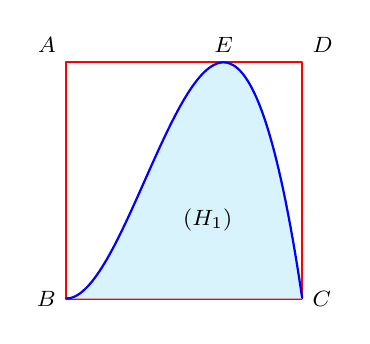
\begin{tikzpicture}[scale=1, font=\footnotesize, line join=round, line cap=round,>=stealth]
			% Khung hình vuông
			\draw[thick, red] (0,3) node[above left, black] {$A$} -- (3,3) node[above right, black] {$D$} -- (3,0) node[right, black] {$C$} -- (0,0) node[left, black] {$B$} -- cycle;			
			\fill[cyan!15] (0,0) -- plot[domain=0:3, samples=100] (\x, {-3/4*(\x)^3 + 9/4*(\x)^2}) -- (3,0) -- cycle;
			\draw[thick, blue] plot[domain=0:3, samples=100] (\x, {-3/4*(\x)^3 + 9/4*(\x)^2});			
			\node[above] at (2,3) {$E$};
			\node at (1.8, 1) {$\left(H_1\right)$};
		\end{tikzpicture}
	}
	\shortans{$394$}
	\loigiai{
		Chọn hệ trục tọa độ $Oxy$ sao cho $B \equiv O(0;0)$.\\
		Khi đó $A(0; 30)$, $C(30; 0)$, $D(30; 30)$.\\
		Vì $AE = 20$ nên $E$ có tọa độ $E(20; 30)$.\\
		Giả sử hàm số bậc ba có đồ thị như hình vẽ là $y = f(x) = ax^3 + bx^2 + cx + d$ ($a \neq 0$).\\
		Ta có $f'(x) = 3ax^2 + 2bx + c$.\\
		Đồ thị hàm số đi qua các điểm $B(0;0)$, $C(30;0)$, $E(20;30)$ và đạt cực đại tại $E(20;30)$. Do đó ta có hệ phương trình
		\[\heva{&f(0) = 0 \\&f(30) = 0 \\&f(20) = 30 \\&f'(20) = 0}
		\Leftrightarrow
		\heva{&	d = 0 \\&27\,000a + 900b + 30c+d = 0 \\&	8\,000a + 400b + 20c+d = 30 \\&
			1\,200a + 40b + c = 0}
		\Leftrightarrow
		\heva{&a = -\dfrac{3}{400} \\&b = \dfrac{9}{40} \\&c = 0 \\&d = 0.}
		\]
		Vậy hàm số bậc ba là $y = -\dfrac{3}{400}x^3 + \dfrac{9}{40}x^2$.\\
		Diện tích phần tô màu $\left(H_1\right)$ là
		\[ S_{H_1} = \displaystyle\int\limits_{0}^{30} \left( -\dfrac{3}{400}x^3 + \dfrac{9}{40}x^2 \right) \mathrm{\,d}x = \left.\left( -\dfrac{3}{1\,600}x^4 + \dfrac{3}{40}x^3 \right) \right|_{0}^{30} = 506{,}25 \text{ m}^2.\]
		Diện tích mảnh đất hình vuông $ABCD$ là $S = 30 \times 30 = 900 \text{ m}^2$.\\
		Diện tích phần còn lại của mảnh đất là $S_{\text{còn lại}} = 900 - 506{,}25=393{,}75\approx 394 \text{ m}^2$.
	}
\end{ex}
%%%=============================%%%

%%%=============EX_18=============%%%
\begin{ex}%[1H8V7-4]%[TDMZZ06]%[Võ Hiệp]
	Cho hình lăng trụ $ABC. A'B'C'$ có đáy $ABC$ là tam giác vuông tại $A$ với $AB=6$, $AC=8$, có tam giác $ABA'$ là tam giác đều. Gọi $M$ là trung điểm của cạnh $AB$, góc giữa hai đường thẳng $A'M$ và $AC$ bằng $60^\circ$. Hãy tính thể tích của khối lăng trụ $ABC. A'B'C'$ (\textit{làm tròn kết quả đến hàng đơn vị}).
	\par
	\shortans{$108$}
	\loigiai{
		\immini{
			Gọi $N$ là trung điểm $BC$. \\
			Ta có $M$ là trung điểm của cạnh $AB$.\\
			Suy ra $MN\parallel AC\Rightarrow MN\perp AB$ (vì $\triangle ABC$ vuông tại $A$).\\
			Lại có $\triangle ABA'$ đều nên $A'M\perp AB$.\\
			Suy ra $AB\perp (A'MN)\Rightarrow (A'MN)\perp (ABC)$.\\
			Trong mặt phẳng $(A'MN)$ kẻ $A'H$ vuông $MN$ tại $H$.\\
			Ta có $\heva{&(A'MN)\perp (ABC)\\& (A'MN)\cap(ABC)=MN\\& A'H\perp MN}\Rightarrow A'H\perp (ABC)$.\\
			Vì $MN\parallel AC$, suy ra $(A'M,AC)=(A'M,MH)=\widehat{HMA'}=60^\circ$.
			
		}{
			\begin{tikzpicture}[scale=1,>=stealth, font=\footnotesize, line join=round, line cap=round]
				\def\a{4}
				\def\h{4.2}
				\path 	(0:0) coordinate (C)
				++(0:\a) coordinate (B)
				++(-135:\a/2) coordinate (A)
				(A)++(100:\h) coordinate (A')
				($(A')+(C)-(A)$) coordinate (C')
				($(C')+(B)-(C)$) coordinate (B')
				($(A)!.5!(B)$) coordinate  (M)
				($(C)!.5!(B)$) coordinate  (N)
				($(M)!.5!(N)$) coordinate  (H); 
				\draw[dashed] (B)--(C) (M)--(N) (A')--(N) (A')--(H);
				\draw (C)--(C') (B)--(B') 	(A)--(A') (A')--(M) (A')--(B)
				(B)--(A)--(C) (A')--(B')--(C')--cycle;
				\foreach \x/\g in {A/-150,B/-30,C/-150,A'/90,B'/30,C'/150,M/-30,N/135,H/-90}
				\fill[black] 	(\x) circle (1pt)
				($(\g:3mm)+(\x)$) node {$\x$};	
				\draw pic[draw,angle radius=2mm]{right angle=B--A--C};
				\draw pic[draw,angle radius=2mm]{right angle=M--H--A'};
				\draw pic[draw,angle radius=3mm]{angle=A'--M--N};
			\end{tikzpicture}
		}
		\noindent
		Tam giác $A'HM$ vuông tại $H$ có $\widehat{HMA'}=60^\circ$, $A'M=AB\cdot\dfrac{\sqrt{3}}{2}= 6\cdot \dfrac{\sqrt{3}}{2}=3\sqrt{3}$.\\
		Suy ra $A'H=\sin \widehat{HMA'}\cdot A'M=\sin 60^\circ \cdot 3\sqrt{3}= \dfrac{\sqrt{3}}{2}\cdot 3\sqrt{3}=\dfrac{9}{2}$.\\
		Thể tích khối lăng trụ
		$V=S_{\triangle ABC}\cdot A'H=\dfrac{1}{2}AB\cdot AC\cdot A'H=\dfrac{1}{2}\cdot 6\cdot 8\cdot \dfrac{9}{2}=108$.
	}
\end{ex}
%%%=============================%%%

%%%=============EX_19=============%%%
\begin{ex}%[2H5V3-4]%[TDMZZ06]%[Nguyễn Đức Tuấn Anh]
	\immini[thm]{
		Trên trần nhà được coi là phẳng song song với mặt đất có bốn điểm $A$, $B$, $C$, $D$ theo thứ tự tạo thành một hình thang vuông tại $A$ và $B$, có các kích thước $AB=40$ cm, $BC=40$ cm, $AD=60$ cm. Người ta dự định đặt mua một quả cầu phong thuỷ $(T)$ rất nặng có bán kính $R$ chưa biết và sẽ sử dụng $4$ đoạn dây không giãn có độ dài $70$ cm, $70$ cm, $60$ cm, $60$ cm lần lượt có một đầu treo vào các điểm $A$, $B$, $C$, $D$ và đầu còn lại gắn vào các điểm trên quả cầu $(T)$. Biết rằng các đoạn dây này đều có đường kéo dài đi qua tâm của $(T)$. Hãy tính theo đơn vị centimet khoảng cách từ điểm thấp nhất của quả cầu $(T)$ đến trần nhà (\textit{làm tròn kết quả đến hàng đơn vị}).}{
		\begin{tikzpicture}[scale=0.7, font=\footnotesize, line join=round, line cap=round, >=stealth]
			\def\R{1.8} % Bán kính quả cầu trên bản vẽ
			\path 
			(0, 4.5) coordinate (A)
			(-3.2, 3.2) coordinate (B)
			(0.8, 1.8) coordinate (C)
			(4.2, 2.5) coordinate (D)
			(0.2, -2.5) coordinate (I)
			($(B)!0.35cm!(A)$) coordinate (B1)
			($(B)!0.35cm!(C)$) coordinate (B2)
			($(B1)+(B2)-(B)$) coordinate (B3);
			\foreach \v in {A, B, C, D} {
				\coordinate (P\v) at ($(I)!\R cm!(\v)$);
			}
			% Đa giác bao quanh lưới ABCD để mô phỏng mặt phẳng trần rộng hơn
			\fill[gray!15] (-5.5, 3.0) -- (-0.5, 6.0) -- (6.5, 3.5) -- (1.5, 0.5) -- cycle;
			% Vẽ viền mờ cho trần nhà để tách biệt không gian
			\draw[gray!40] (-5.5, 3.0) -- (-0.5, 6.0) -- (6.5, 3.5) -- (1.5, 0.5) -- cycle;
			\draw (A) -- (B) -- (C) -- (D) -- cycle;
			\draw (A) -- (PA) (B) -- (PB) (C) -- (PC) (D) -- (PD);
			% Quả cầu 
			\shade[ball color=black!90] (I) circle (\R);
			\fill[white, opacity=0.5, rounded corners=1pt] ($(I) + (-1.1, -0.6)$) rectangle ++(0.3, 0.4);
			\fill[white, opacity=0.5, rounded corners=1pt] ($(I) + (-0.7, -0.6)$) rectangle ++(0.15, 0.4);
			\fill[white, opacity=0.15] ($(I) + (0.3, 0.8)$) ellipse (0.8 and 0.4);
			% Ghi chú 
			\foreach \u/\v/\txt/\pos in {A/B/$AB=40$\,cm/above, A/D/$AD=60$\,cm/above, B/C/$BC=40$\,cm/above} {
				\path (\u) -- (\v) node[midway, sloped, \pos] {\txt};
			}
			\foreach \v/\txt/\pos/\x in {A/$70$\,cm/below/0.65, B/$70$\,cm/below/0.5, C/$60$\,cm/below/0.5, D/$60$\,cm/below/0.5} {
				\path (\v) -- (P\v) node[pos=\x, sloped, \pos] {\txt};
			}
			\foreach \v/\pos in {A/above, B/left, C/above, D/right} {
				\fill (\v) circle (1.2pt) node[\pos] {\v};}
			\foreach \x/\y/\z in {D/A/B,C/B/A} \draw pic[draw,angle radius=2mm]
			{right angle= \x--\y--\z};
		\end{tikzpicture}
	}
	\par\shortans{$168$}
	\loigiai{
		\begin{center}
			\begin{tikzpicture}[scale=0.8, font=\footnotesize, line join=round, line cap=round, >=stealth,	x={(-0.6cm,-0.4cm)}, y={(1cm,0cm)}, z={(0cm,1cm)}]
				\fill[gray!10, opacity=0.8] (-1.5,-1.5,0) -- (6,-1.5,0) -- (6,8,0) -- (-1.5,8,0) -- cycle;
				\draw[gray!40] (-1.5,-1.5,0) -- (6,-1.5,0) -- (6,8,0) -- (-1.5,8,0) -- cycle;
				\draw[->] (0,0,0) -- (6.5,0,0) node[below] {$x$};
				\draw[->] (0,0,0) -- (0,7.5,0) node[right] {$y$};
				\draw[->] (0,0,0) -- (0,0,1.5) node[above] {$z$};
				\draw[dashed] (0,0,0)--(0,0,-4.5);
				\coordinate (A) at (0,0,0);
				\coordinate (B) at (4,0,0);
				\coordinate (C) at (4,4,0);
				\coordinate (D) at (0,6,0);
				\draw[] (A) -- (B) -- (C) -- (D) -- cycle;
				\coordinate (I) at (2.5, 3, -5); 
				\coordinate (H) at (2.5, 3, 0);
				\draw (B) -- (I) (C) -- (I) (D) -- (I);
				\draw[dashed] (A) -- (I) ;
				\foreach \p/\pos/\txt in {A/above right/$A \equiv O$, B/above left/$B$, C/above/$C$, D/above/$D$, I/below/$I$} {
					\fill (\p) circle (1.5pt) node[\pos] {\txt};
				}
				\draw pic[draw,angle radius=2.5mm] {right angle= D--A--B};
				\draw pic[draw,angle radius=2.5mm] {right angle= A--B--C};
				\path (A) -- (B) node[midway, sloped, below] {$40$};
				\path (B) -- (C) node[midway, sloped, below] {$40$};
				\path (A) -- (D) node[midway, sloped, above] {$60$};
			\end{tikzpicture}
		\end{center}
		Chọn hệ trục tọa độ $Oxyz$ sao cho mặt phẳng $(Oxy)$ trùng với mặt phẳng trần nhà, gốc tọa độ $O$ trùng với $A$.\\
		Vì $ABCD$ là hình thang vuông tại $A$ và $B$ nên $AD \parallel BC$, $AB \perp AD$ và $AB \perp BC$.\\
		Với các kích thước $AB=40$\,cm, $BC=40$\,cm, $AD=60$\,cm, ta có tọa độ các điểm là $A(0;0;0)$, $B(40;0;0)$, $C(40;40;0)$, $D(0;60;0)$.\\
		Gọi $I(x;y;z)$ là tâm của quả cầu $(T)$. Do quả cầu treo dưới trần nhà nên $z < 0$. Gọi $h = -z > 0$ là khoảng cách từ $I$ đến trần nhà, ta có $I(x;y;-h)$.\\
		Do các đoạn dây kéo dài đi qua tâm quả cầu nên khoảng cách từ các điểm treo đến tâm $I$ bằng tổng độ dài dây và bán kính $R$ của quả cầu.\\
		Ta có hệ phương trình
		\[	\heva{
			&IA^2 = (70+R)^2 \\
			&IB^2 = (70+R)^2 \\
			&IC^2 = (60+R)^2 \\
			&ID^2 = (60+R)^2
		} \Leftrightarrow \heva{
			&x^2 + y^2 + h^2 = (70+R)^2 \quad &(1) \\
			&(x-40)^2 + y^2 + h^2 = (70+R)^2 \quad &(2) \\
			&(x-40)^2 + (y-40)^2 + h^2 = (60+R)^2 \quad &(3) \\
			&x^2 + (y-60)^2 + h^2 = (60+R)^2. \quad &(4)
		}\]
		Từ $(1)$ và $(2)$ suy ra $x^2 = (x-40)^2 \Leftrightarrow 2x = 40 \Leftrightarrow x = 20$.\\
		Từ $(3)$ và $(4)$ suy ra
		\begin{eqnarray*}
			&&(20-40)^2 + (y-40)^2 + h^2 = 20^2 + (y-60)^2 + h^2 \\
			&\Leftrightarrow& (y-40)^2 = (y-60)^2\\
			&\Leftrightarrow& y-40 = -(y-60) \\
			&\Leftrightarrow& y = 50.
		\end{eqnarray*}
		Thay $x=20$, $y=50$ vào $(1)$ và $(4)$, ta được
		\[\heva{
			&20^2 + 50^2 + h^2 = (R+70)^2 \\
			&20^2 + (50-60)^2 + h^2 = (R+60)^2
		} \Leftrightarrow \heva{
			&h^2 + 2\,900 = R^2 + 140R + 4\,900 \\
			&h^2 + 500 = R^2 + 120R + 3\,600.
		}\]
		Trừ vế theo vế hai phương trình trên, ta có
		\[2\,400 = 20R + 1\,300 \Leftrightarrow 20R = 1\,100 \Leftrightarrow R = 55.\]
		Thay $R=55$ vào phương trình thứ hai, ta có
		\[h^2 + 500 = (55+60)^2 \Leftrightarrow h^2 = 12\,725 \Rightarrow h = \sqrt{12\,725}.\]
		Khoảng cách từ điểm thấp nhất của quả cầu $(T)$ đến trần nhà bằng
		\[d = h + R = \sqrt{12\,725} + 55 \approx 168 \text{ (cm)}.\]
	}
\end{ex}
%%%=============================%%%

%%%=============EX_20=============%%%
\begin{ex}%[0D0C2-3]%[TDMZZ06]%[Lê Hồ Quang Minh]
	Xếp ngẫu nhiên $24$ cuốn sách Tinh Hoa Công Phá Đề Toán giống nhau vào $16$ ngăn sách được bố trí như hình vẽ. Gọi $p$ là xác suất để có đúng $4$ ô để trống và các ô trống này \textbf{không} kề nhau (hai ô được gọi là kề nhau nếu có chung một cạnh). Hãy tính $10^5\cdot p$ \textit{(làm tròn kết quả đến hàng đơn vị)}.
	\shortans[oly]{$2420$}
	\begin{center}
		\begin{tikzpicture}[scale=0.8, line join=round, line cap=round]
			\draw[thick] (0,0) rectangle (2,8);
			\draw[thick] (1,0) -- (1,8);
			\foreach \y in {1,2,3,4,5,6,7} {
				\draw (0,\y) -- (2,\y);	}
			\draw[<->] (-0.5,0) -- (-0.5,8) node[midway, left] {$8$ ngăn};
			\draw[<->] (0,-0.5) -- (2,-0.5) node[midway, below] {$2$ cột};
		\end{tikzpicture}
	\end{center}
	\loigiai{
		Xếp $24$ cuốn sách giống nhau vào $16$ ngăn khác nhau tương đương với bài toán tìm số nghiệm nguyên không âm của phương trình $x_1 + x_2 + \dots + x_{16} = 24$.\\
		Do đó, số phần tử của không gian mẫu $$n(\Omega)=\mathrm{C}_{24+16-1}^{16-1} = \mathrm{C}_{39}^{15}.$$
		Gọi $A$ là biến cố \lq\lq Có đúng $4$ ô trống và các ô trống này \textbf{không} kề nhau\rq\rq.\\
		Để có đúng $4$ ô trống, ta thực hiện qua $2$ công đoạn:
		\begin{itemize}
			\item \textbf{Công đoạn 1:} Chọn $4$ ô trống trong $16$ ô sao cho không có $2$ ô nào kề cạnh.
			\begin{itemize}
				\item \textbf{Trường hợp 1:} Chọn $1$ cột, trong cột đó chọn $4$ ngăn \textbf{không} cạnh nhau.
				
				Số cách chọn là $\mathrm{C}_2^1 \cdot \mathrm{C}_5^4 = 10$ cách.
				\item \textbf{Trường hợp 2:} Chọn $1$ cột, trong cột đó chọn $3$ ngăn \textbf{không} cạnh nhau, ngăn còn lại thuộc cột còn lại.
				
				Số cách chọn là $\mathrm{C}_2^1\cdot \mathrm{C}_6^3 \cdot 5 = 200$ cách.
				\item \textbf{Trường hợp 3:} Mỗi cột có $2$ ngăn không cạnh nhau
				\begin{itemize}
					\item \textbf{Trường hợp 3.1:}
					
					Chọn $2$ ô trống nằm ở $2$ đầu của cột thứ nhất có $1$ cách chọn.
					
					Chọn $2$ ô trống \textbf{không} cạnh nhau ở $6$ vị trí chính giữa của cột còn lại có $\mathrm{C}_5^2$ cách.
					
					Số cách chọn là $\mathrm{C}_5^2 = 10$ cách.
					\item \textbf{Trường hợp 3.2:}
					
					Chọn $1$ ô trống ở đầu hoặc cuối và $1$ ô trống bên trong của cột thứ nhất có $2 \cdot 5 = 10$ cách.
					
					Chọn $2$ ô trống ở cột còn lại có $\mathrm{C}_6^2 - 4 = 11$ cách.
					
					Số cách chọn là $10 \cdot 11 = 110$ cách.
					\item \textbf{Trường hợp 3.3:}
					
					Chọn $2$ ô trống \textbf{không} cạnh nhau bên trong của cột thứ nhất có $\mathrm{C}_5^2 = 10$ cách.
					
					Chọn $2$ ô trống ở cột còn lại có $\mathrm{C}_7^2 - 9 = 12$ cách.
					
					Số cách chọn là $10 \cdot 12 = 120$ cách.
				\end{itemize}
				Như vậy, \textbf{Trường hợp 3} có tất cả $240$ cách.
			\end{itemize}
			\item \textbf{Công đoạn 2:} Xếp $24$ cuốn sách vào $12$ ô còn lại sao cho mỗi ô có ít nhất $1$ cuốn sách.\\
			Số cách xếp là $\mathrm{C}_{12+12-1}^{12-1} = \mathrm{C}_{23}^{11}$.
		\end{itemize}
		Suy ra $n(A) = \left(10 + 200 + 240\right) \cdot \mathrm{C}_{23}^{11} = 450 \cdot \mathrm{C}_{23}^{11}$.\\
		Do đó xác suất cần tìm là $p = \dfrac{n(A)}{n(\Omega)} = \dfrac{450 \cdot \mathrm{C}_{23}^{11}}{\mathrm{C}_{39}^{15}} = \dfrac{805}{33\,263}$. \\
		Vậy $10^5 p \approx 2\,420$.
	}
\end{ex}
%%%=============================%%%

%%%=============EX_21=============%%%
\begin{ex}%[2D4C3-5]%[TDM31]%[Nguyễn Văn Sang]
	\immini[thm]
	{Cho một khối đặc có dạng hình nón $(N)$ như hình vẽ, với bán kính đường tròn đáy bằng $20$\,cm và chiều cao bằng $50$\,cm. Dùng một mặt phẳng song song với đường thẳng $SA$ để cắt $(N)$ sẽ cho ta thiết diện là một parabol có diện tích là $F$. Hãy tính theo đơn vị centimet vuông giá trị lớn nhất của $F$ \textit{(làm tròn kết quả đến hàng đơn vị)}.
	}
	{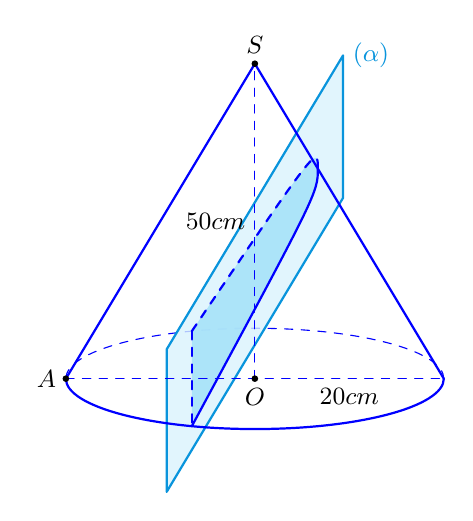
\begin{tikzpicture}[>=stealth, scale=0.8, font=\small, line join=round, line cap=round]
			% 1. Đáy nón (phần khuất)
			\draw[dashed, blue] (3,0) arc (0:180:3 and 0.8);
			
			% 2. Mặt phẳng cắt (alpha) - vẽ dưới dạng fill mờ để thấy các đường nét bên trong
			\coordinate (V1) at (-1.4, 0.465);
			\coordinate (V2) at (-1.4, -1.797);
			\coordinate (V3) at (1.4, 2.869);
			\coordinate (V4) at (1.4, 5.131);
			\fill[cyan!15, opacity=0.8] (V1) -- (V2) -- (V3) -- (V4) -- cycle;
			
			% Tọa độ các điểm cắt thiết diện
			\coordinate (M) at (-1, 0.754);
			\coordinate (N) at (-1, -0.754);
			\coordinate (K) at (1, 3.333);
			
			% 3. Thiết diện parabol
			\fill[cyan!35, opacity=0.9] (M) .. controls (1, 3.71) .. (K) .. controls (1, 2.956) .. (N) -- cycle;
			\draw[dashed, thick, blue] (M) .. controls (1, 3.71) .. (K); % Nét khuất của parabol
			\draw[dashed, thick, blue] (M) -- (N); % Dây cung cắt đáy (nằm ở đáy)
			
			% 4. Các đường viền của mặt phẳng alpha
			\draw[cyan!80!blue, thick] (V1) -- (V2) -- (V3) -- (V4) -- cycle;
			\node[cyan!80!blue, right] at (V4) {$(\alpha)$};
			
			% 5. Đáy nón (phần thấy)
			\draw[blue, thick] (-3,0) arc (180:360:3 and 0.8);
			
			% 6. Nét thấy của parabol
			\draw[thick, blue] (N) .. controls (1, 2.956) .. (K); 
			
			% 7. Thân nón và các đường dóng
			\draw[thick, blue] (-3,0) -- (0,5) -- (3,0);
			\draw[dashed, blue] (-3,0) -- (3,0);
			\draw[dashed, blue] (0,0) -- (0,5);
			
			% 8. Điểm và Nhãn
			\node[above] at (0,5) {$S$};
			\node[left] at (-3,0) {$A$};
			\node[below] at (0,0) {$O$};
			\fill (0,5) circle (1.5pt);
			\fill (-3,0) circle (1.5pt);
			\fill (0,0) circle (1.5pt);
			
			% 9. Kích thước
			\node[left] at (0,2.5) {$50\text{ cm}$};
			\node[below] at (1.5,0) {$20\text{ cm}$};
	\end{tikzpicture}}
	\par\shortans[0]{$933$}
	\loigiai{
		\immini
		{\begin{itemize}
				\item Gọi bán kính đáy nón là $R = 20\text{ cm}$.
				\item Chiều cao $SO = h = 50\text{ cm}$.
				\item Độ dài đường sinh $SA$ là
				\[ l = SA = \sqrt{R^2 + h^2} = \sqrt{20^2 + 50^2} = 10\sqrt{29} \text{ (cm)}.\]
				\item Gọi mặt phẳng cắt hình nón là $(P)$. Vì $(P) \parallel SA$, $(P)$ cắt mặt đáy theo một dây cung $MN$ vuông góc với đường kính $AB$ (với $A, O, B$ thẳng hàng). Gọi $I$ là giao điểm của $MN$ và $AB$.
		\end{itemize}}
		{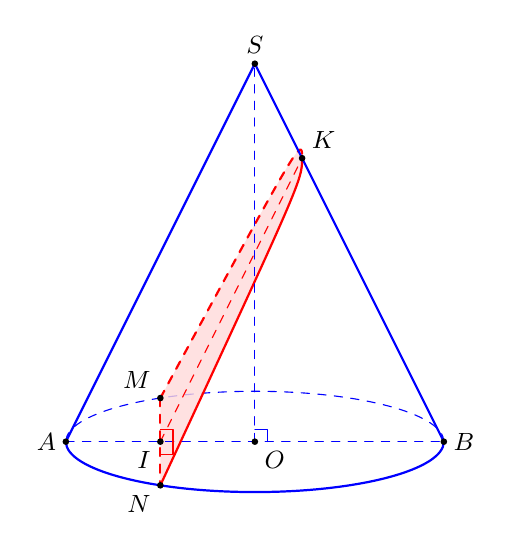
\begin{tikzpicture}[>=stealth, scale=0.8, font=\small, line join=round, line cap=round]
				% Định nghĩa các hằng số tỷ lệ
				\def\R{3}    
				\def\h{6}    
				\def\b{0.8}  
				
				% Vẽ elip đáy (phần khuất)
				\draw[dashed, thin, blue] (\R,0) arc (0:180:\R cm and \b cm);
				
				% Các điểm chính
				\coordinate (A) at (-\R,0);
				\coordinate (B) at (\R,0);
				\coordinate (S) at (0,\h);
				\coordinate (O) at (0,0);
				
				% Vị trí I 
				\def\xI{-1.5}
				\coordinate (I) at (\xI,0);
				
				% Tọa độ M, N
				\def\yMN{0.6928} 
				\coordinate (M) at (\xI, \yMN); 
				\coordinate (N) at (\xI, -\yMN); 
				
				% Đỉnh K của Parabol
				\coordinate (K) at (0.75, 4.5);
				
				% Đổ màu thiết diện Parabol
				\fill[red!15, opacity=0.8] (M) .. controls (0.75, 4.846) .. (K) .. controls (0.75, 4.154) .. (N) -- cycle;
				
				% Vẽ elip đáy (phần thấy)
				\draw[thick, blue] (-\R,0) arc (180:360:\R cm and \b cm);
				
				% Các đường nét bên trong
				\draw[dashed, thick, red] (M) -- (N); % Dây cung MN
				\draw[dashed, thin, red] (I) -- (K); % Trục IK
				
				% Vẽ biên Parabol tách biệt nét đứt/nét liền tạo hiệu ứng 3D
				\draw[dashed, thick, red] (M) .. controls (0.75, 4.846) .. (K); % Cung phía sau (khuất)
				\draw[thick, red] (N) .. controls (0.75, 4.154) .. (K); % Cung phía trước (thấy)
				
				% Biên và trục khối nón
				\draw[thick, blue] (A) -- (S) -- (B);
				\draw[dashed, thin, blue] (A) -- (B);
				\draw[dashed, thin, blue] (O) -- (S);
				
				% --- Ký hiệu góc vuông ---
				\draw[blue, thin] (0.2, 0) -- (0.2, 0.2) -- (0, 0.2); % Góc vuông tại O
				\draw[red, thin] (-1.3, 0) -- (-1.3, 0.2) -- (-1.5, 0.2); % Góc vuông tại I (nửa trên)
				\draw[red, thin] (-1.3, 0) -- (-1.3, -0.2) -- (-1.5, -0.2); % Góc vuông tại I (nửa dưới)
				
				% Nhãn và điểm
				\node[above] at (S) {$S$};
				\node[left] at (A) {$A$};
				\node[right] at (B) {$B$};
				\node[below right] at (O) {$O$};
				\node[above right] at (K) {$K$};
				\node[below left] at (I) {$I$};
				\node[above left] at (M) {$M$};
				\node[below left] at (N) {$N$};
				
				\fill (S) circle (1.5pt);
				\fill (A) circle (1.5pt);
				\fill (B) circle (1.5pt);
				\fill (O) circle (1.5pt);
				\fill (K) circle (1.5pt);
				\fill (I) circle (1.5pt);
				\fill (M) circle (1.5pt);
				\fill (N) circle (1.5pt);
		\end{tikzpicture}}
		\begin{itemize}
			\item Đặt đoạn $AI = x$ với điều kiện $x \in (0; 40)$. Khi đó $BI = AB - AI = 40 - x$.
			\item Thiết diện cắt bởi mặt phẳng $(P)$ là một parabol có đỉnh $K$ nằm trên đường sinh $SB$, nhận $IK$ làm trục đối xứng và $IK \parallel SA$.
			\item Xét $\Delta SAB$, vì $IK \parallel SA$, áp dụng định lý Ta-lét ta có
			\[ \dfrac{IK}{SA} = \dfrac{BI}{BA} \Rightarrow IK = SA \cdot \dfrac{BI}{BA} = 10\sqrt{29} \cdot \dfrac{40 - x}{40} = \dfrac{\sqrt{29}}{4}(40 - x).\]
			Chiều cao của parabol chính là độ dài đoạn $IK$.
			\item Xét đường tròn đáy, dây cung $MN \perp AB$ tại $I$, áp dụng hệ thức lượng ta có
			\[ MI^2 = AI \cdot BI = x(40 - x) \Rightarrow MN = 2 \cdot MI = 2\sqrt{x(40 - x)}.\]
			Độ dài dây cung đáy của parabol là $MN$.
			\item Diện tích thiết diện parabol là hàm số $F(x)$
			\begin{align*}
				F(x) &= \dfrac{2}{3} \cdot MN \cdot IK \\
				&= \dfrac{2}{3} \cdot 2\sqrt{x(40 - x)} \cdot \dfrac{\sqrt{29}}{4}(40 - x) \\
				&= \dfrac{\sqrt{29}}{3} \sqrt{x(40 - x)^3}.
			\end{align*}
			\item Để $F(x)$ lớn nhất, ta xét hàm số $g(x) = x(40 - x)^3$ trên khoảng $(0; 40)$.
			\item Tính đạo hàm
			\begin{align*}
				g'(x) &= 1 \cdot (40 - x)^3 + x \cdot 3(40 - x)^2 \cdot (-1) \\
				&= (40 - x)^2 \big[ (40 - x) - 3x \big] \\
				&= (40 - x)^2 (40 - 4x).
			\end{align*}
			\item Cho $g'(x) = 0 \Leftrightarrow \hoac{&40 - x = 0 \\ &40 - 4x = 0} \Leftrightarrow \hoac{&x = 40 \text{ (loại)} \\ &x = 10 \text{ (nhận.)}}$
			\item Bảng biến thiên của hàm số $g(x)$ trên khoảng $(0; 40)$
			\begin{center}
				
\begin{tikzpicture}
					\tkzTabInit[lgt=1.5,espcl=3.5,deltacl=0.5]
					{$x$ / 1, $g'(x)$ / 1, $g(x)$ / 2}
					{$0$, $10$, $40$}
					\tkzTabLine{ , +, 0, -, }
					\tkzTabVar{-/ $0$, +/ $270\,000$, -/ $0$}
				\end{tikzpicture}
			\end{center}
			\item Dựa vào bảng biến thiên, $\displaystyle \max_{(0; 40)} g(x) = g(10) = 10 \cdot (40 - 10)^3 = 270\,000$.
			\item Do đó, diện tích lớn nhất của thiết diện là
			\[ F_{\max} = \dfrac{\sqrt{29}}{3} \cdot \sqrt{270\,000} = \dfrac{\sqrt{29}}{3} \cdot 300\sqrt{3} = 100\sqrt{87} \approx 933 \text{ (cm}^2\text{)}.\]
		\end{itemize}
	}
\end{ex}
%%%=============================%%%

%%%=============EX_22=============%%%
\begin{ex}%[0D0C2-6]%[TDM42]%[Unknown]
	Cho hình đa giác đều $(H)$ gồm có $36$ đỉnh và có bán kính đường tròn ngoại tiếp bằng $11$. Chọn ngẫu nhiên $8$ đỉnh từ các đỉnh của $(H)$.
	\begin{center}
		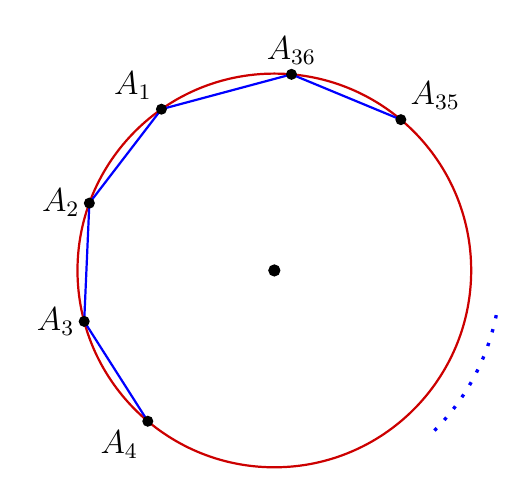
\begin{tikzpicture}[scale=1]
			\def\R{2.5}
			\draw[red!80!black, thick] (0,0) circle (\R);
			\filldraw[black] (0,0) circle (2pt);
			\coordinate (A35) at (50:\R);
			\coordinate (A36) at (85:\R);
			\coordinate (A1) at (125:\R);
			\coordinate (A2) at (160:\R);
			\coordinate (A3) at (195:\R);
			\coordinate (A4) at (230:\R);
			\draw[blue, thick] (A35) -- (A36) -- (A1) -- (A2) -- (A3) -- (A4);
			\tikzstyle{point}=[circle, fill=black, inner sep=0pt, minimum size=4pt]
			\node[point] at (A35) {};
			\node[above right, font=\large] at (A35) {$A_{35}$};
			\node[point] at (A36) {};
			\node[above, font=\large] at (A36) {$A_{36}$};
			\node[point] at (A1) {};
			\node[above left, font=\large] at (A1) {$A_1$};
			\node[point] at (A2) {};
			\node[left, font=\large] at (A2) {$A_2$};
			\node[point] at (A3) {};
			\node[left, font=\large] at (A3) {$A_3$};
			\node[point] at (A4) {};
			\node[below left, font=\large] at (A4) {$A_4$};
			\draw[blue, very thick, loosely dotted] (-45:1.15*\R) arc (-45:-10:1.15*\R);
		\end{tikzpicture}
	\end{center}
	Gọi $p$ là xác suất để chọn được bát giác có đúng $3$ cạnh có độ dài nhỏ hơn $4$. Hãy tính $10^4 p$ (\textit{làm tròn kết quả đến hàng đơn vị}).
	\par
	\shortans[0]{$3638$}
	\loigiai{
		\textbf{1. Không gian mẫu}\\
		Phép thử: Chọn ngẫu nhiên $8$ đỉnh từ $36$ đỉnh của đa giác đều để tạo thành một bát giác. \\
		Số phần tử của không gian mẫu là $n(\Omega) = \mathrm{C}_{36}^8 = 30\,260\,340$.
		
		\textbf{2. Phân tích điều kiện cạnh của bát giác}\\
		Giả sử hai đỉnh của bát giác cách nhau $x$ cung (với $1 \le x \le 36-7 = 29$, $x \in \mathbb{N}^*$).\\
		Góc ở tâm chắn cung này là $\varphi = x \cdot \dfrac{2\pi}{36} = \dfrac{x\pi}{18}$.\\
		Độ dài cạnh của bát giác nối hai đỉnh đó là:
		$$L = 2R \sin\left(\dfrac{\varphi}{2}\right) = 2 \cdot 11 \cdot \sin\left(\dfrac{x\pi}{36}\right)$$
		Yêu cầu cạnh có độ dài nhỏ hơn $4$:
		$$22 \sin\left(\dfrac{x\pi}{36}\right) < 4 \Leftrightarrow \sin\left(\dfrac{x\pi}{36}\right) < \dfrac{2}{11} \approx 0{,}1818$$
		Vì $x \ge 1$ nên ta có $\dfrac{x\pi}{36} < \arcsin\left(\dfrac{2}{11}\right) \approx 0{,}1828 \text{ rad} \Rightarrow x < \dfrac{36 \cdot 0{,}1828}{\pi} \approx 2{,}09$.\\
		Do $x$ là số nguyên dương nên $x \in \{1; 2\}$.\\
		Vậy cạnh của bát giác có độ dài $<4$ khi và chỉ khi nó chắn $1$ hoặc $2$ cung của đa giác đều ban đầu.
		
		\textbf{3. Đếm số kết quả thuận lợi}\\
		Gọi $x_1, x_2, \ldots, x_8$ là số cung của đa giác đều nằm giữa các đỉnh liên tiếp của bát giác. Khi đó:
		\begin{equation}
			x_1 + x_2 + x_3 + \dots + x_8 = 36 \quad (1)
		\end{equation}
		với $x_i \in \mathbb{N}^*$ và $x_i$ chính là khoảng cách cung ứng với mỗi cạnh của bát giác.\\
		Yêu cầu bài toán tương đương với: Trong $8$ biến $x_i$, có \textbf{đúng $3$ biến} nhận giá trị thuộc tập $\{1; 2\}$, và $5$ biến còn lại nhận giá trị $\ge 3$.\\
		Số cách chọn $3$ vị trí (trong $8$ vị trí cạnh) cho $3$ biến nhận giá trị nhỏ là $\mathrm{C}_8^3$.\\
		Giả sử $3$ biến đó là $x_1, x_2, x_3 \in \{1; 2\}$ và $x_4, x_5, x_6, x_7, x_8 \ge 3$. Ta xét các trường hợp của tổng $3$ biến nhỏ $S_3 = x_1 + x_2 + x_3$:
		
		\begin{itemize}
			\item \textbf{Trường hợp 1:} Cả $3$ biến đều bằng $1 \Rightarrow x_1=x_2=x_3=1$. (Có $1$ cách)\\
			Tổng $5$ biến còn lại: $x_4 + x_5 + \dots + x_8 = 36 - 3 = 33$ (với $x_i \ge 3$).\\
			Đặt $y_i = x_i - 2 \ge 1$, ta có $y_4 + y_5 + \dots + y_8 = 33 - 5 \times 2 = 23$.\\
			Số nghiệm nguyên dương của phương trình này là $\mathrm{C}_{23-1}^{5-1} = \mathrm{C}_{22}^4$.\\
			$\Rightarrow$ Số dãy thỏa mãn TH này là: $1 \cdot \mathrm{C}_{22}^4$.
			
			\item \textbf{Trường hợp 2:} Có $2$ biến bằng $1$, $1$ biến bằng $2 \Rightarrow S_3 = 4$. (Có $\mathrm{C}_3^1 = 3$ hoán vị)\\
			Tổng $5$ biến còn lại: $x_4 + x_5 + \dots + x_8 = 36 - 4 = 32$.\\
			Phương trình đổi biến: $y_4 + y_5 + \dots + y_8 = 32 - 10 = 22$.\\
			Số nghiệm là $\mathrm{C}_{21}^4$.\\
			$\Rightarrow$ Số dãy thỏa mãn TH này là: $3 \cdot \mathrm{C}_{21}^4$.
			
			\item \textbf{Trường hợp 3:} Có $1$ biến bằng $1$, $2$ biến bằng $2 \Rightarrow S_3 = 5$. (Có $\mathrm{C}_3^1 = 3$ hoán vị)\\
			Tổng $5$ biến còn lại: $x_4 + x_5 + \dots + x_8 = 36 - 5 = 31$.\\
			Phương trình đổi biến: $y_4 + y_5 + \dots + y_8 = 31 - 10 = 21$.\\
			Số nghiệm là $\mathrm{C}_{20}^4$.\\
			$\Rightarrow$ Số dãy thỏa mãn TH này là: $3 \cdot \mathrm{C}_{20}^4$.
			
			\item \textbf{Trường hợp 4:} Cả $3$ biến đều bằng $2 \Rightarrow x_1=x_2=x_3=2$. (Có $1$ cách)\\
			Tổng $5$ biến còn lại: $x_4 + x_5 + \dots + x_8 = 36 - 6 = 30$.\\
			Phương trình đổi biến: $y_4 + y_5 + \dots + y_8 = 30 - 10 = 20$.\\
			Số nghiệm là $\mathrm{C}_{19}^4$.\\
			$\Rightarrow$ Số dãy thỏa mãn TH này là: $1 \cdot \mathrm{C}_{19}^4$.
		\end{itemize}
		
		Tổng số dãy $(x_1, x_2, \dots, x_8)$ thỏa mãn bài toán là:
		$$M = \mathrm{C}_8^3 \left( \mathrm{C}_{22}^4 + 3\mathrm{C}_{21}^4 + 3\mathrm{C}_{20}^4 + \mathrm{C}_{19}^4 \right)$$
		$$M = 56 \left( 7\,315 + 3 \cdot 5\,985 + 3 \cdot 4\,845 + 3\,876 \right) = 56 \times 43\,681 = 2\,446\,136$$
		
		Mỗi cách chọn $1$ bát giác tương ứng với việc chọn điểm bắt đầu trên đường tròn. Do đa giác có $36$ đỉnh và bát giác có $8$ đỉnh, nên số bát giác thực tế được tạo ra (tránh lặp do phép quay vòng) theo nguyên lý điểm bắt đầu là:
		$$n(A) = \dfrac{36}{8} \times M = \dfrac{36}{8} \times 2\,446\,136 = 11\,007\,612$$
		
		\textbf{4. Tính xác suất}\\
		Xác suất cần tìm là:
		$$p = \dfrac{n(A)}{n(\Omega)} = \dfrac{11\,007\,612}{\mathrm{C}_{36}^8} = \dfrac{11\,007\,612}{30\,260\,340}.$$
		Vậy $10^4 p \approx 3\,638$.
	}
\end{ex}
%%%=============================%%%